\documentclass[12pt,a4paper]{article}
\usepackage[utf8x]{inputenc}
\usepackage[russian]{babel}
\usepackage[OT1]{fontenc}
\usepackage{amsmath}
\usepackage{amsfonts}
\usepackage{amssymb}
\usepackage{indentfirst}
%%%% Graphics
\usepackage[dvipsnames]{xcolor}			% driver-independent color 
\usepackage{wrapfig}						% produces figures which text can flow around

\usepackage{fancyvrb}
\usepackage{graphicx}
\usepackage{xcolor}
\usepackage{textcomp}
\usepackage{listings}
\lstset{
	breaklines=true, % Перенос длинных строк
	basicstyle=\ttfamily\footnotesize, % Шрифт для отображения кода
	frame=tblr % draw a frame at all sides of the code block
	tabsize=2, % tab space width
	showstringspaces=false, % don't mark spaces in strings
	% Настройка отображения номеров строк
	numbersep=5pt, % Отступ от кода
}
\renewcommand{\lstlistingname}{Листинг}
\usepackage{titlesec}
\usepackage{amsmath} % American Mathematical Society (AMS) math facilities
\usepackage{amsfonts} % fonts from the AMS
\usepackage{amssymb}	 % additional math symbols
\usepackage{amscd}
\usepackage{latexsym}
\setlength{\parskip}{1em}
\usepackage[left=2.5cm, right=1.5cm, top=1.5cm, bottom=1.5cm]{geometry}
\setlength{\parindent}{0.5cm}
\newcommand{\sectionbreak}{\clearpage}
\author{Федор Кусов\\<fdr91@mail.ru>}
\title{Отчет по лабораторной работе 1: \\\LaTeX{}, Git, GPG}
\begin{document}
\maketitle
\newpage
\tableofcontents{}
\section{Cистема верстки \TeX{} и расширения \LaTeX{}}
\subsection{Цель работы}
Изучение принципов верстки TEX, создание первого отчета
\subsection{Ход работы}
\subsubsection{Создание минимального файла .tex в простом текстовом редакторе – преамбула, тело документа}


Документ LaTeX — это текстовый файл, содержащий специальные команды языка разметки. Документ делится на преамбулу и тело.

Преамбула содержит информацию про класс документа, использованные пакеты макросов, определения макросов, автора, дату создания документа и другую информацию. Ниже представлена простая преамбула для статьи
\begin{Verbatim}[xleftmargin=.5in,fontsize=\small]
\documentclass[12pt]{article} % Класс документа article, величина шрифта 12пт.
\usepackage[russian]{babel} % Пакет поддержки русского языка
\title{Отчет по лабораторной работе 1: \Latex{} Git GPG} % Заглавие документа
\date{\today} % Дата создания
\end{Verbatim}

Тело документа содержит текст документа и команды разметки. Оно должно находиться между командами $\backslash$begin\{document\} и $\backslash$end\{document\}.
\subsubsection{Компиляция в командной строке – latex, xdvi, pdflatex}
Работа с файлами на языке latex осуществляется при помощи пакета утилит. Вот некоторые из них:
\begin{itemize}
\item latex -- принимает файл на языке \LaTeX{} на вход, выдавая бинарный файл в формате dvi (от DeVice independent -- независимый от устройства). Пример использования:
\begin{Verbatim}[xleftmargin=.5in,fontsize=\small]
latex report.tex
\end{Verbatim}

Результатом работы команды будет файл report.dvi
\item xdvi -- позволяет вывести содержимое .dvi на экран
\begin{Verbatim}[xleftmargin=.5in,fontsize=\small]
xdvi report.dvi
\end{Verbatim}
Выведет report.dvi на экран в графическом виде.
\item pdflatex -- преобразует .tex в формат PDF.
\begin{Verbatim}[xleftmargin=.5in,fontsize=\small]
pdflatex report.tex
\end{Verbatim}
Преобразует report.tex в report.pdf
\end{itemize}
\subsubsection{Оболочка TexMaker, Быстрый старт, Быстрая сборка}
Texmaker представляет собой редактор текста и исходного кода LaTeX. TexMaker предоставляет доступ к утилитам LaTeX посредством графического интерфейса (GUI) Развитый GUI позволяет ускорить работу с документами за счет таких функций, как автодополнение, быстрое создание документов из шаблонов и т.д.

Быстрый старт (Quick Start) в TexMaker -- это мастер для создания новых документов, позволяющий задать основные параметры документа, подключить нужные модули.

Быстрая сборка (Quick Build) специальная кнопка, к которой можно привязать выполнение последовательности команд для сборки и отображения документа. 
\subsubsection{Создание титульного листа, нескольких разделов, списка, несложной формулы}
Титульный лист в LaTeX можно быстро создать командой $\backslash$maketitle. В шаблон листа при этому будут подставлены такие сведения, как имя автора, учебное заведение, название работы.
 
Для создания раздела используется команда $\backslash$section, принимающая название раздела в качестве документа. Подразделы и подподразделы создаются при помощи $\backslash$subsection и $\backslash$subsubsection соответственно.

Для создания списка служит пара команд $\backslash$begin{itemize} и $\backslash$end{itemize}. Записи в списке задаются при помощи команды $\backslash$item.

LaTeX имеет средства для быстрого написания математических формул. Примеры написания простых формул:
\begin{itemize}
\item Индексы:
\begin{verbatim}Верхние a^b
\end{verbatim}
\begin{verbatim}Нижние a^b
\end{verbatim}
\item Дроби:
\begin{verbatim}a/b
\end{verbatim}
\item Скобки:
\begin{verbatim}(a) [] \{a\}
\end{verbatim}
\end{itemize}

Возможно записать и более сложные формулы. Например, следующая строка: \begin{center}
\begin{verbatim}
\iiint_{x^2+y^2+z^2=1} f(x,y,z) dx dy dz
\end{verbatim}
\end{center}

Даст на выходе:
\begin{center}
$\iiint_{x^2+y^2+z^2=1} f(x,y,z) dx dy dz $
\end{center}
\subsubsection{Понятие классов документов, подключаемых пакетов}
Каждый документ в LaTeX начинается с команды \verb+\documentclass[...]{…}+в фигурных скобках которой задаются параметры оформления стиля документа, а в квадратных — список классовых опций.

В LaTeX существует 5 основных классов документов: 
\begin{itemize}
\item article -- статья,
\item report -- небольшая книга, статья, разбитая на главы
\item book -- книга,
\item proc -- возможно использовать для докладов
\item letter -- деловое письмо. 
\end{itemize}

Помимо этих основных, есть ещё множество дополнительных классов, таких как beamer.

Пакеты в позволяют расширять, если это требуется, возможности LaTeX. Для подключения пакетов используется команда \verb+\usepackage[опции]{пакет}+.

Некоторые пакеты включены в стандартную установку LaTeX. Другие можно поставить отдельно. Информацию о существующих пакетах можно получить при помощи The LaTeX Companion.
\subsection{Выводы}

Рассмотрим систему LaTeX с точки зрения её достоинств и недостатков.

Недостатки:
\begin{itemize}
\item сложность изучения -- LaTeX сложно использовать и изучать одновременно. Изучение требует сознательного обучения.
\item создание новых стилей оформления -- сложная задача. Как правило, обычные пользователи не в силах с ней справиться
\end{itemize}

Достоинства:
\begin{itemize}
\item Высокое качество результата, недоступное другим средствам полиграфической подготовки (верстки) текстов.
\item Гибкость
\item Простота подготовки очень сложных документов самым неискушенным пользователем.
\item Большое количество макропакетов, позволяющих сделать все, что угодно.
\item Низкие системные требования.
\item Высокая переносимость - один и тот же результат на любой технике.
\item Поддержка любых языков в рамках одного документа.
\item Строгий подход к оформлению удерживает пользователя в рамках полиграфических приличий.
\item Удобная работа с математическими формулами
\item Пользователь должен знать всего несколько легко запоминающихся команд, которые определяют логическую структуру документа, и почти не должен знать о том, как документ форматируется.
\item Сложные элементы текста, такие как сноски, библиография, оглавление, список таблиц и т.п., а также простые рисунки могут быть выполнены без особых трудностей.
\end{itemize}

Первое знакомство с LaTeX оставило приятное впечатление. Если сравнивать LaTeX с Microsoft Word, при решении таких задач, как, например, написание выпускной работы бакалавра, создается впечатление, что LaTeX позволил бы гораздо меньшими усилиями написать хорошо структурированную работу, соответствующую ГОСТам, правильно оформить рисунки, таблицы, формулы,список литературы и сноски.
\section{Система контроля версий Git}
\subsection{Цель работы}
Изучить систему контроля версий Git, освоить основные приемы работы
с ней.
\subsection{Ход работы}
\subsubsection{Изучить справку для основных команд}
Справка для основных команд была изучена автором ранее при работе над студенческими проектами с использованием Github для хранения версий.
\subsubsection{Получить содержимое репозитория}
Для получения содержимого репозиторию используется команда clone
\begin{verbatim}git clone https://github.com/fdr91/InfoSecCourse2015
\end{verbatim}
\subsubsection{Добавить новую папку и первый файл под контроль версий}
Для этого может быть использована последовательность команд:
\begin{verbatim}mkdir folder
git add folder
echo 1 > folder/file.txt
git add folder/file.txt\end{verbatim}
\subsubsection{Зафиксировать изменения в локальном репозитории}
\begin{verbatim}git commit -m "Add folder/file.txt under version control"
\end{verbatim}
\subsubsection{Внести изменения в файл и просмотреть различия}
\begin{verbatim}echo 2 >> foder/file.txt
git diff folder/file.txt
\end{verbatim}
\subsubsection{Отменить локальные изменения}
\begin{verbatim}git checkout
\end{verbatim}
\subsubsection{Внести изменения в файл и просмотреть различия}
\begin{verbatim}echo 2 >> foder/file.txt
git diff folder/file.txt
\end{verbatim}
\subsubsection{Зафиксировать изменения в локальном репозитории, зафиксировать изменения в центральном репозитории}
\begin{verbatim}git commit -m "Add changes to folder/file.txt"
git push
\end{verbatim}
\subsubsection{Получить изменения из центрального репозитория}
\begin{verbatim}git commit -m "Add changes to folder/file.txt"
git pull
\end{verbatim}
\subsubsection{Поэкспериментировать с ветками}
\begin{verbatim}
git checkout -b branch
echo 3 >> folder/file.txt && git add folder/file.txt
git commit -m "folder/file.txt modified. Again"
git checkout master
git merge branch
git branch -d branch
\end{verbatim}
\subsection{Выводы}

Git является широкораспространенной системой контроля версий. Автору уже не раз приходилось работать с ней в рамках работы над различными студенческими проектами. Git удобен и прост в использовании. Бесплатный хостинг репозиториев GitHub делает Git доступным благодаря простоте создания собственного репозитория и наличию web-интерфейса для работы с контролем версий и багтрекинга.

Основные преимущества распределённых систем — их гибкость и значительно большая (по сравнению с централизованными системами) автономия отдельного рабочего места. Каждый компьютер разработчика является, фактически, самостоятельным и полнофункциональным сервером, из таких компьютеров можно построить произвольную по структуре и уровню сложности систему, задав (как техническими, так и административными мерами) желаемый порядок синхронизации. При этом каждый разработчик может вести работу независимо, так, как ему удобно, изменяя и сохраняя промежуточные версии документов, пользуясь всеми возможностями системы (в том числе доступом к истории изменений) даже в отсутствие сетевого соединения с сервером. Связь с сервером или другими разработчиками требуется исключительно для проведения синхронизации, при этом обмен наборами изменений может осуществляться по различным схемам.
\section{Программа для шифрования и подписи GPG,пакет Gpg4win}
\subsection{Цель работы}
Научиться создавать сертификаты, шифровать файлы и ставить ЭЦП.
\subsection{Ход работы}
\subsubsection{ Изучить документацию, запустить графическую оболочку Kleopatra}
Kleopatra -- это менеджер сертификатов, который позволяет работать с GPG. Он предоставляет графический интерфейс для работы с GPG.
\subsubsection{Создать ключевую пару OpenPGP}
Для создания ключевой пары используется команда File → New Certificate. Информация о созданном сертификате отображается на вкладке My Certificates.
\begin{figure}[h!]
\centering
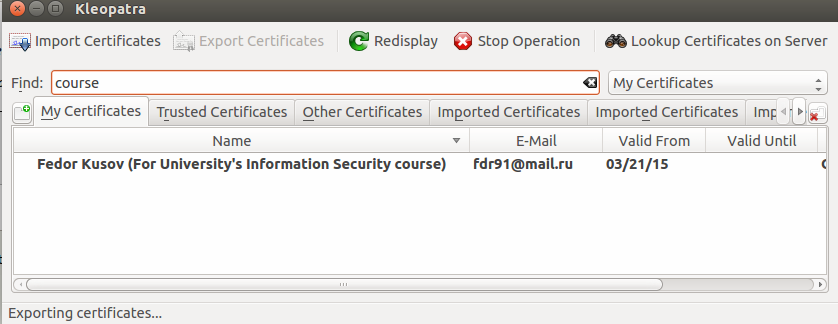
\includegraphics[scale=0.6]{resources/kleo_sertificates.png}
\caption{Созданный сертификат}
\end{figure}
\subsubsection{Экспортировать сертификат}
Экспорт сертификата осуществляется командой File → Export Certificate В листинге 1. Представлено содержимое файла-сертификата.
\lstinputlisting[language={},caption={Сертификат в формате asc (ASCII Armored file)}]{resources/4D993562416D9E8330C3EB759619A14BB00B243C.asc}
\subsubsection{Поставить ЭЦП на файл}
Для того, чтобы поставить ЭЦП на файл, используется команда File → Sign/Encrypt Files. Результатом выполнения станет появление файла с расширением .sig.
\subsubsection{Получить чужой сертификат из репозитория, файл с данными и файл с сигнатурой (подписью)}
В качестве чужого сертификата был использован сертификат Семена Мартынова из репозитория  https://github.com/SemenMartynov/InfoSecCourse2015
\subsubsection{Импортировать сертификат, подписать его}
Импортирование осуществляется командой File → Import Certificates. Импортированый сертификат отображается во вкладке Imported Certificates
\begin{figure}[h!]
\centering
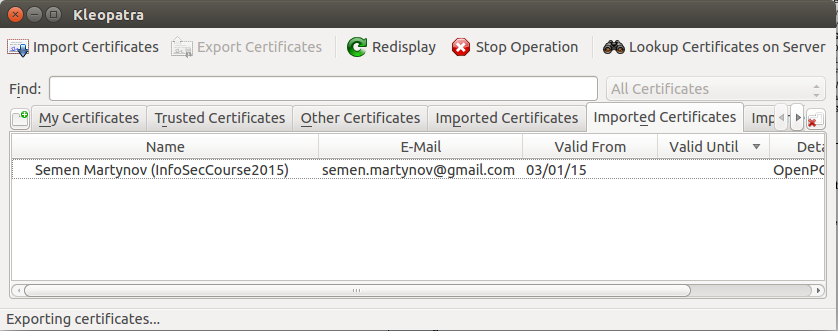
\includegraphics[scale=0.6]{resources/is.png}
\caption{Импортированный сертификат}
\end{figure}
Импортированный сертификат нужно подписать. Для этого нужно: Щелкнуть правой кнопкой мышью на сертификате  →  Certify Certificate
В открывшемся окне нужно поставить флажок "I have verified the fingerprint".
\begin{figure}[h!]
\centering
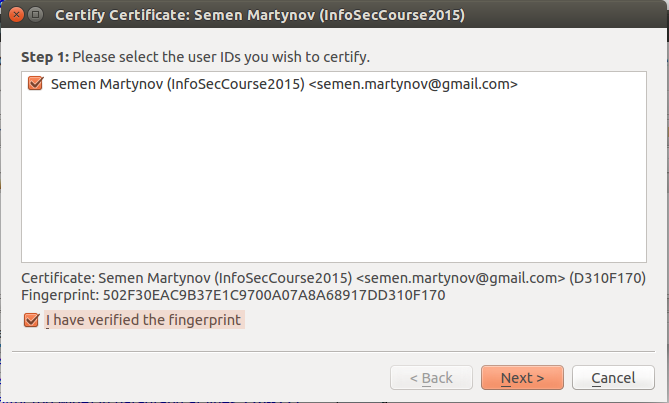
\includegraphics[scale=0.6]{resources/ss.png}
\caption{Импортированный сертификат}
\end{figure}
\subsubsection{Проверить подпись}
Для проверки сертификата используется команда File → Verify Certificate.
\subsubsection{Используя GNU Privacy handbook потренироваться в использовании gpg через интерфейс командной строки, без использования графических оболочек}
Результат, полученный при помощи Kleopatra легко повторить используя терминал. Генерация ключа происходит в диалоговом режиме после ввода команды
\begin{verbatim}gpg --gen-key
\end{verbatim}
В процессе работы, мастер создания ключа запросит следующую информацию:
\begin{itemize}
	\item{Тип ключа (по умолчанию это DSA и ElGamal).}
	\item{Размер ключа (с DSA/ElGamal ключами не использую длину больше чем 2048).}
	\item{"срок годности" ключа.}
	\item{Информацию о пользователе (имя, электронный адрес).}
	\item{Пароль для ключа (если нужен).}
\end{itemize}

В процессе генерации ключа, GnuPG использует энтропию. Для способствования её сбору рекомендуется активно двигать мышкой или запустить mp3 в фоновом режиме.

Просмотреть доступные в системе ключи позволяет команда
\begin{verbatim}gpg --list-keys
\end{verbatim}
Её вывод показан на рисунке 7.

Для экспорта можно использовать команду
\begin{verbatim}gpg --armor --output john.asc --export john@mail.ru
\end{verbatim}

Для импорта используется
\begin{verbatim}gpg --import tomas.asc
\end{verbatim}
\end{document}